% Preámbulo
\documentclass[12pt, aspectratio = 169]{beamer}
    % Paquetes
    \usepackage[spanish]{babel}
    \usepackage{lipsum}
    \usepackage{xcolor}
    
    
    % Temas
    %\usetheme{Madrid}
    %\usetheme{CambridgeUS}
    \usetheme{JuanLesPins}
        \usecolortheme{default}
        \definecolor{verde}{RGB}{34,139,34}
        \setbeamercolor{structure}{fg = verde}
        

    % Carátula - título
    \title{Presentación II}
    \author{Jhon R. Ordoñez}
    \date{\today}
% Cuerpo del documento
\begin{document}
    % Carátula
    \begin{frame}
        \maketitle
    \end{frame}
    % Contenido
    \begin{frame}{Contenido}
        \tableofcontents
    \end{frame}
    % Sección 1
    \section{Introducción}
        % Slide 1.1
        \begin{frame}[t]
            \frametitle{Introducción} \pause
            \begin{enumerate}
                \item Primavera \pause
                \item Verano \pause
                \item Otoño \pause
                \item Invierno.
            \end{enumerate}
        \end{frame}
    % Sección 2
    \section{Marco teórico}
         % Slide 2.1
        \begin{frame}[t]
            \frametitle{Marco teórico}
            \begin{enumerate}[<+->]
                \item Marco histórico
                \item Marco teórico
                \item Marco conceptual
                \item Marco referencial
            \end{enumerate}
        \end{frame}
    % Sección 3
    \section{Metodología}
         % Slide 3.1
        \begin{frame}[t]
            \frametitle{Seasons}
            \begin{enumerate}[<+->]
                \item Summer
                \item Autumn
                \item Winter
                \item Spring.
            \end{enumerate}
        \end{frame}
        % Slide 3.2
        \begin{frame}[<+->][t]
            \frametitle{Animals}
            \begin{itemize}
                \item Cow
                \item Goat
            \end{itemize}
            %
            \begin{itemize}
                \item Lion
                \item Tiger
            \end{itemize}
        \end{frame}
        % Slide 3.3
        \begin{frame}[t]
            \frametitle{Seasons}
            \begin{enumerate}[<+-|alert@+>]
                \item Summer
                \item Autumn
                \item Winter
                \item Spring.
            \end{enumerate}
        \end{frame}
    % Sección 4
    \section{Entornos BEAMER}
        % Slide 4.1
        \begin{frame}[t]
            \begin{block}{Rule}
                The amsmath and amssymb ...
            \end{block}
        %
            \begin{alertblock}<2->{Warning}
                A mathematical expression ...
            \end{alertblock}
        %
            \begin{exampleblock}{Example}<3>
                $\sin^2\theta + \cos^2\theta = 1$
            \end{exampleblock}
        \end{frame}
        % Slide 4.2
        \begin{frame}[t]
            \begin{theorem}
                $(a+b)^2=a^2 + 2ab + b^2$
            \end{theorem}
            %
            \begin{proof}<2->
                $(a+b)^2=(a+b)(a+b)=a^2+2ab+b^2$
            \end{proof}
            %
            \begin{example}<3->[Square of sum]
                $(3+5)^2=3^2+2\times3\times5+5^2=64$
            \end{example}
        \end{frame}
    
    % Sección 5
    \section{Tablas}
        % Slide 5.1
        \begin{frame}{Tablas}
            \begin{table}
                \flushleft
                \begin{tabular}{cccc}
                    \hline & {\bf Total} & {\bf Passed} & {\bf Pass rate}\\
                    \hline Boys & 56 & 50 & 89.3\%\\
                    Girls & 38 & 36 & 94.7\%\\
                    \hline
                \end{tabular}
            \end{table}
        \end{frame}
        
    % Sección 6
    \section{Columnas}
        % Slide 6.1
        \begin{frame}
            \frametitle{Page layout}
            How a page … below:\pause\vskip 5mm
            \begin{columns}
            \column{0.4\textwidth}
                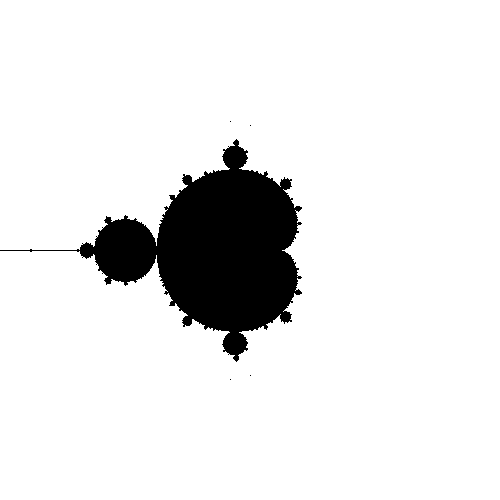
\includegraphics[width=\textwidth]{image4.png}
            %
            \column{0.6\textwidth}
                \begin{itemize}[<+-|alert@+>]
                    \item A page is composed of different …
                    \item Components are specified in length …
                    \item Length of a component can be …
                \end{itemize}
            \end{columns}
        \end{frame}
    % Sección 7
    \section{Vínculos}
        % Slide 7.1
        \begin{frame}[t,label = Slide 7.1]
            \frametitle{Page layout}
            How a page layout is composed is shown below:\pause \vskip 5mm
            \begin{columns}
            \column{0.4\textwidth}
                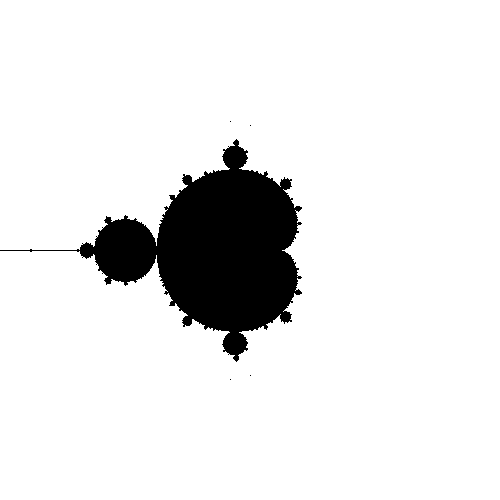
\includegraphics[width=\textwidth]{image4.png}
            %
            \column{0.45\textwidth}
                \begin{itemize}[<+-|alert@+>]
                    \item A page is composed \hfill
                    \hyperlink{Slide 7.2}{\beamerreturnbutton{Volver}}
                    \item Components
                    \item Length 
                \end{itemize}
            \end{columns}
        \end{frame}

        % Slide 7.2
        \begin{frame}[t,label = Slide 7.2]
            \begin{itemize}[<+-|alert@+>]
                \frametitle{\LaTeX\ components}
                \item Font selection
                \item Formatting Texts
                \item Page layout \hfill \hyperlink{Slide 7.1}{\beamergotobutton{Ver la figura}}
                \item Table, figure, equation, etc.
            \end{itemize}
        \end{frame}
    % Bibliografía
    \begin{frame}{Bibliografía}
        \bibliography{biblio}
        \bibliographystyle{apalike}
            % Autores
            \nocite{cameron-2010}
    \end{frame}
    % Carátula
    \begin{frame}
        \maketitle
    \end{frame}
    % Apéndice
    
    
\end{document}




